% !TEX program = xelatex
\documentclass[UTF8,zihao=-4,oneside,openany]{ctexbook}

% Shared style for the combined handout.  Section files keep standalone
% preambles for now, while the master document uses this single definition.
\usepackage[a4paper,top=20mm,bottom=22mm,left=19mm,right=19mm,headheight=24pt]{geometry}
\usepackage[table]{xcolor}
\usepackage{amsmath,amssymb,mathtools,bm}
\usepackage{siunitx}
\usepackage{booktabs,tabularx,array,multicol}
\usepackage{enumitem}
\usepackage{tikz}
\usetikzlibrary{arrows.meta,positioning,calc,angles,quotes,patterns}
\usepackage[most]{tcolorbox}
\usepackage{fancyhdr}
\usepackage{hyperref}

\definecolor{Ink}{HTML}{202326}
\definecolor{DeepBlue}{HTML}{294E69}
\definecolor{Blue}{HTML}{47687D}
\definecolor{PaleBlue}{HTML}{F3F5F6}
\definecolor{Gold}{HTML}{6E777D}
\definecolor{PaleGold}{HTML}{F6F6F5}
\definecolor{Green}{HTML}{5B6D76}
\definecolor{PaleGreen}{HTML}{F3F5F6}
\definecolor{Alert}{HTML}{666B6F}
\definecolor{PaleAlert}{HTML}{F6F6F6}
\definecolor{RuleGray}{HTML}{D3D7DA}
\definecolor{TextGray}{HTML}{61686D}
\definecolor{SoftGray}{HTML}{F6F6F6}

\color{Ink}
\sisetup{
  per-mode=symbol,
  inter-unit-product=\ensuremath{{}\cdot{}},
  exponent-product=\times
}

\hypersetup{
  colorlinks=true,
  linkcolor=DeepBlue,
  urlcolor=Blue,
  pdfsubject={高中物理竞赛一轮资料重排讲义},
  pdfauthor={物理竞赛一轮资料编写组}
}

\setlength{\parindent}{2em}
\setlength{\parskip}{0.25em}
\setlist{nosep,leftmargin=2em}
\setcounter{secnumdepth}{3}
\setcounter{tocdepth}{2}
\numberwithin{equation}{section}
\counterwithin{table}{section}
\allowdisplaybreaks[2]
\emergencystretch=2em

\ctexset{
  chapter={
    format=\raggedright\LARGE\bfseries\color{Ink},
    titleformat=\LARGE\bfseries\color{Ink},
    beforeskip=0pt,
    afterskip=18pt
  },
  section={
    format=\Large\bfseries\color{DeepBlue},
    beforeskip=1.8ex,
    afterskip=1.0ex
  },
  subsection={
    format=\large\bfseries\color{Ink},
    beforeskip=1.5ex,
    afterskip=0.8ex
  },
  subsubsection={format=\normalsize\bfseries\color{Ink}}
}

\pagestyle{fancy}
\fancyhf{}
\fancyhead[L]{\small\color{TextGray}高中物理竞赛一轮讲义}
\fancyhead[R]{\small\color{TextGray}第一章\quad 数学与物理工具}
\fancyfoot[C]{\small\color{TextGray}\thepage}
\renewcommand{\headrulewidth}{0.4pt}
\renewcommand{\headrule}{\hbox to\headwidth{\color{RuleGray}\leaders\hrule height \headrulewidth\hfill}}

\newcommand{\dimens}[1]{\operatorname{dim}\!\left(#1\right)}
\newcommand{\dd}{\mathop{}\!\mathrm{d}}
\newcommand{\vect}[1]{\bm{#1}}
\newcommand{\uvec}[1]{\hat{\vect{#1}}}
\newcommand{\e}{\mathrm e}
\newcommand{\order}[1]{\mathcal O\!\left(#1\right)}
\DeclareMathOperator{\proj}{proj}
\newcommand{\examplesource}[1]{%
  \par{\small\color{TextGray}题源：#1}\par
}

\newtcolorbox{goalbox}{
  enhanced,breakable,
  colback=PaleBlue,colframe=Blue,
  boxrule=0.7pt,arc=2mm,
  title={本节目标},fonttitle=\bfseries,
  coltitle=DeepBlue,
  attach boxed title to top left={xshift=5mm,yshift=-2mm},
  boxed title style={colback=white,colframe=Blue,boxrule=0.7pt,arc=1.5mm}
}

\newtcolorbox{sourcebox}{
  enhanced,breakable,
  colback=SoftGray,colframe=RuleGray,
  boxrule=0.5pt,arc=0mm,
  title={题源说明},fonttitle=\bfseries,
  coltitle=Ink,colbacktitle=SoftGray,
  borderline west={1.2pt}{0pt}{TextGray}
}

\newtcolorbox[auto counter,number within=section]{examplebox}[2][]{
  enhanced,breakable,
  colback=white,colframe=RuleGray,
  boxrule=0.5pt,arc=0mm,
  title={例题~\thetcbcounter\quad #2},fonttitle=\bfseries,
  coltitle=Ink,colbacktitle=PaleBlue,
  borderline west={1.4pt}{0pt}{DeepBlue},
  #1
}

\newtcolorbox{methodbox}[1]{
  enhanced,breakable,
  colback=PaleBlue,colframe=RuleGray,
  boxrule=0.5pt,arc=0mm,
  title={方法：#1},fonttitle=\bfseries,
  coltitle=Ink,colbacktitle=PaleBlue,
  borderline west={1.2pt}{0pt}{DeepBlue}
}

\newtcolorbox{warningbox}[1]{
  enhanced,breakable,
  colback=SoftGray,colframe=RuleGray,
  boxrule=0.5pt,arc=0mm,
  title={易错提醒：#1},fonttitle=\bfseries,
  coltitle=Ink,colbacktitle=SoftGray,
  borderline west={1.2pt}{0pt}{TextGray}
}

\newtcolorbox{extensionbox}[1]{
  enhanced,breakable,
  colback=PaleGold,colframe=Gold,
  boxrule=0.5pt,arc=0mm,
  title={拓展：#1},fonttitle=\bfseries,
  coltitle=Ink,colbacktitle=PaleGold,
  borderline west={1.2pt}{0pt}{DeepBlue}
}

\newtcolorbox{summarybox}{
  enhanced,breakable,
  colback=PaleBlue,colframe=DeepBlue,
  boxrule=0.9pt,arc=1.5mm,
  title={本节小结},fonttitle=\bfseries,
  coltitle=white,colbacktitle=DeepBlue
}

\newtcolorbox{exercisebox}[1]{
  enhanced,breakable,
  colback=white,colframe=RuleGray,
  boxrule=0.7pt,arc=1.5mm,
  title={#1},fonttitle=\bfseries,
  coltitle=DeepBlue,colbacktitle=PaleBlue
}

\tikzset{
  vector/.style={-{Latex[length=2.5mm]},very thick,draw=DeepBlue},
  component/.style={-{Latex[length=2.2mm]},thick,draw=TextGray},
  axis/.style={-{Latex[length=2mm]},thin,draw=TextGray},
  guide/.style={densely dashed,draw=TextGray},
  curve/.style={very thick,draw=DeepBlue},
  tangent/.style={thick,draw=TextGray},
  secant/.style={thick,draw=DeepBlue}
}

\usetikzlibrary{decorations.pathmorphing}
\newcommand{\Needspace}[1]{%
  \par
  \ifdim\dimexpr\pagegoal-\pagetotal\relax<#1\relax
    \newpage
  \fi
}

\newif\ifwithsolutions
\ifdefined\NOSOLUTIONS
  \withsolutionsfalse
\else
  \withsolutionstrue
\fi

\ifwithsolutions
  \hypersetup{
    pdftitle={学而思物理竞赛一轮资料重排：第四章第一节 功与功率，动能定理（含补写解答与解图）},
    pdfsubject={学而思物理竞赛一轮资料重排；正文与例题据原资料整理，解答与解图为后补},
    pdfauthor={原资料：学而思；重排与补写解答：物理竞赛一轮资料编写组}
  }
\else
  \hypersetup{
    pdftitle={学而思物理竞赛一轮资料重排：第四章第一节 功与功率，动能定理},
    pdfsubject={学而思物理竞赛一轮资料原版重排；无解答版},
    pdfauthor={原资料：学而思；重排：物理竞赛一轮资料编写组}
  }
\fi

\fancyhead[R]{\small\color{TextGray}第四章\quad 功和动能，机械能守恒}
\renewcommand{\theequation}{\thechapter.\arabic{equation}}

\newtcolorbox{origexamplebox}[1]{
  enhanced,breakable,
  colback=white,colframe=RuleGray,
  boxrule=0.5pt,arc=0mm,
  title={#1},fonttitle=\bfseries,
  coltitle=Ink,colbacktitle=PaleBlue,
  borderline west={1.4pt}{0pt}{DeepBlue}
}

\NewDocumentEnvironment{xesolution}{+b}{%
  \ifwithsolutions
    \par\smallskip
    \begingroup\small
    \noindent{\bfseries\color{DeepBlue}解答}\quad #1
    \par\endgroup\medskip
  \fi
}{}

% Technical geometry and labels share one coordinate system per panel.
\tikzset{solbody/.style={draw=Ink,line width=.8pt},solpath/.style={draw=Ink,line width=.8pt},
 solforce/.style={-{Latex[length=2mm]},draw=DeepBlue,line width=.9pt},
 solflow/.style={-{Latex[length=1.8mm]},draw=Blue,line width=.8pt},
 solgeom/.style={draw=TextGray,densely dashed,line width=.5pt},
 sollabel/.style={font=\scriptsize,fill=none,inner sep=1.5pt},
 solpanel/.style={font=\scriptsize\bfseries,text=TextGray},
 spring/.style={decorate,decoration={coil,segment length=4pt,amplitude=2.5pt},draw=Ink}}
\newcommand{\diagcaption}[2]{\refstepcounter{figure}\par\nopagebreak[4]\smallskip
 {\centering\scriptsize\color{TextGray}图~\thefigure\quad #2\par}\smallskip}
\newenvironment{workfig}{\begin{center}\begin{minipage}{.98\linewidth}\centering}{\end{minipage}\end{center}}

\newcommand{\workDerivationDiagram}{%
\begin{workfig}\begin{tikzpicture}[scale=.9]
 \node[solpanel] at (1.6,2.8) {(a) 轨迹与切向速度};
 \draw[solpath,domain=0:2.7,samples=60] plot (\x,{.25*\x*\x});
 \coordinate (A) at (.5,.0625); \coordinate (B) at (1.5,.5625);
 \fill (A) circle (1.6pt) node[below,sollabel] {$A$};
 \fill (B) circle (1.6pt);\node[sollabel] at (1.4,1) {$B$};
 \draw[solforce] (A)--++(1,.25) node[below right,sollabel] {$\vec v_A$};
 \draw[solforce] (B)--++(1,.75) node[right,sollabel] {$\vec v_B$};
 \draw[solforce] (A)--++(0,1.3) node[left,sollabel] {$\vec a_A$};
 \draw[TextGray] ($(A)+(14.036:.45)$) arc(14.036:90:.45);
 \node[sollabel] at ($(A)+(53:.68)$) {$\theta$};
 \begin{scope}[xshift=5cm]
 \node[solpanel] at (1.2,2.8) {(b) 精确的速度矢量关系};
 \coordinate (P) at (0,0); \coordinate (Q) at (2,.5); \coordinate (S) at (2,1.5);
 \draw[solforce] (P)--(Q) node[midway,below,sollabel] {$\vec v_A$};
 \draw[solforce] (P)--(S) node[midway,above left,sollabel] {$\vec v_B$};
 \draw[solforce] (Q)--(S) node[midway,right,sollabel] {$\Delta\vec v$};
 \node[sollabel] at (1,-.7) {$\vec v_B=\vec v_A+\Delta\vec v$};
 \end{scope}
\end{tikzpicture}\diagcaption{示意图}{速度沿轨迹切线；速度增量是两个速度矢量之差。}
\label{ch08:fig:workDerivationDiagram}\end{workfig}}

\newcommand{\probdiagFourOne}{%
\begin{workfig}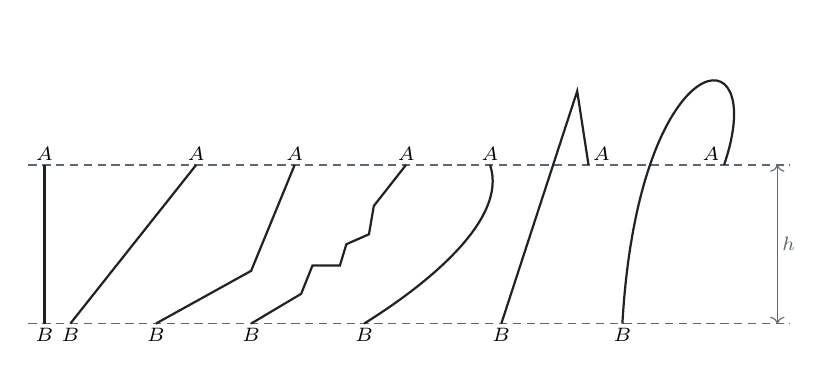
\begin{tikzpicture}[xscale=.82,yscale=.72]
 \draw[solgeom](-.25,2.8)--(11.55,2.8);\draw[solgeom](-.25,0)--(11.55,0);
 \foreach \x in {0,2.35,3.875,5.6,6.9}{\node[sollabel,above]at(\x,2.8){$A$};}
 \node[sollabel,above right]at(8.425,2.8){$A$};\node[sollabel,above left]at(10.525,2.8){$A$};
 \foreach \x in {0,.4,1.725,3.2,4.95,7.075,8.95}{\node[sollabel,below]at(\x,0){$B$};}
 \draw[solpath](0,2.8)--(0,0);
 \draw[solpath](2.35,2.8)--(.4,0);
 \draw[solpath](3.875,2.8)--(3.2,.93)--(1.725,0);
 \draw[solpath](5.6,2.8)--(5.1,2.075)--(5.025,1.575)--(4.675,1.4)--(4.575,1.025)--(4.15,1.025)--(3.975,.525)--(3.2,0);
 \draw[solpath](6.9,2.8)..controls(7.2,1.8)and(5.8,.6)..(4.95,0);
 \draw[solpath](7.075,0)--(8.25,4.1)--(8.425,2.8);
 \draw[solpath](8.95,0)..controls(9.2,5.0)and(11.25,5.2)..(10.525,2.8);
 \draw[<->,TextGray](11.35,0)--(11.35,2.8)node[midway,right,sollabel]{$h$};
\end{tikzpicture}\diagcaption{题图}{七条路径的始末高度差都为 $h$。}\label{ch08:fig:probdiagFourOne}\end{workfig}}

\newcommand{\soldiagFourOne}{%
\begin{workfig}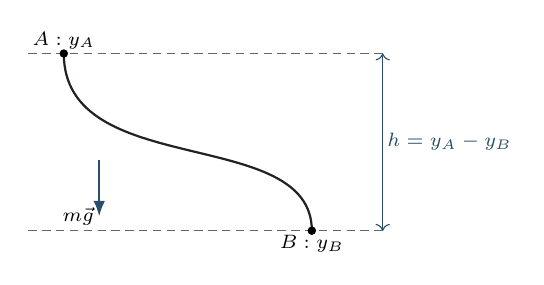
\begin{tikzpicture}[scale=.9]
 \draw[solgeom] (-2,1.5)--(3,1.5);\draw[solgeom] (-2,-1)--(3,-1);
 \draw[solpath] (-1.5,1.5)..controls(-1.5,-.3)and(2,.5)..(2,-1);
 \fill (-1.5,1.5) circle(1.7pt) node[above,sollabel] {$A:y_A$};
 \fill (2,-1) circle(1.7pt) node[below,sollabel] {$B:y_B$};
 \draw[solforce] (-1,0)--(-1,-.8) node[left,sollabel] {$m\vec g$};
 \draw[<->,DeepBlue] (3,-1)--(3,1.5) node[midway,right,sollabel] {$h=y_A-y_B$};
\end{tikzpicture}\diagcaption{解图}{重力功的积分只保留竖直坐标的始末差。}\label{ch08:fig:soldiagFourOne}\end{workfig}}

\newcommand{\probdiagFourTwo}{%
\begin{workfig}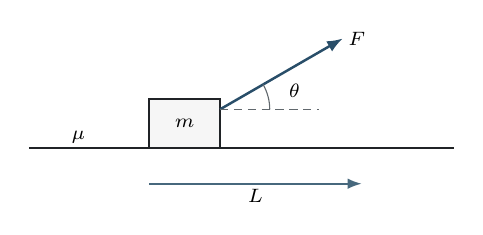
\begin{tikzpicture}[scale=.9]
 \draw[solbody] (-2.2,0)--(3.8,0);
 \draw[solbody,fill=SoftGray] (-.5,0) rectangle (.5,.7);\node[sollabel] at (0,.35) {$m$};
 \draw[solforce] (.5,.55)--++(30:2) node[right,sollabel] {$F$};
 \draw[solgeom] (.5,.55)--(1.9,.55);
 \draw[TextGray] (1.2,.55) arc(0:30:.7);\node[sollabel] at (1.55,.81) {$\theta$};
 \node[sollabel,above] at (-1.5,0) {$\mu$};
 \draw[solflow] (-.5,-.5)--(2.5,-.5) node[midway,below,sollabel] {$L$};
\end{tikzpicture}\diagcaption{题图}{力 $F$ 向右上方，物体沿水平面向右滑动。}\label{ch08:fig:probdiagFourTwo}\end{workfig}}

\newcommand{\soldiagFourTwo}{%
\begin{workfig}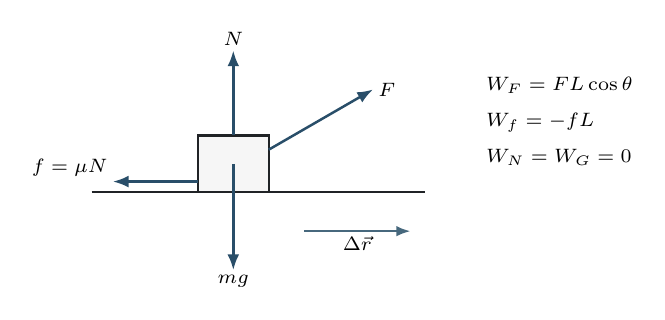
\begin{tikzpicture}[scale=.9]
 \draw[solbody] (-2,0)--(2.7,0);\draw[solbody,fill=SoftGray] (-.5,0) rectangle(.5,.8);
 \draw[solforce] (.5,.6)--++(30:1.7) node[right,sollabel] {$F$};
 \draw[solforce] (0,.8)--(0,2) node[above,sollabel] {$N$};
 \draw[solforce] (0,.4)--(0,-1.1) node[below,sollabel] {$mg$};
 \draw[solforce] (-.5,.15)--(-1.7,.15) node[above left,sollabel] {$f=\mu N$};
 \draw[solflow] (1,-.55)--(2.5,-.55) node[midway,below,sollabel] {$\Delta\vec r$};
 \node[sollabel,align=left,anchor=west] at (3.5,1) {$W_F=FL\cos\theta$\\[5pt]$W_f=-fL$\\[5pt]$W_N=W_G=0$};
\end{tikzpicture}\diagcaption{解图}{竖直方向合力为零；各力作功须与水平位移配对。}\label{ch08:fig:soldiagFourTwo}\end{workfig}}

\newcommand{\probdiagFourThree}{%
\begin{workfig}\begin{tikzpicture}[scale=.85]
 \coordinate(O) at (0,1.8);\coordinate(A) at (2.4,1.8);\coordinate(B) at (0,-1.4);
 \draw[spring] (O)--(A);\draw[spring] (O)--(B);
 \fill (O) circle(2pt) node[above left,sollabel] {$O$};\fill(A)circle(3pt)node[right,sollabel]{$A$};
 \fill(B)circle(3pt)node[below,sollabel]{$B$};
 \node[sollabel] at (1.2,2.15) {$l_0,\ k$};\node[sollabel] at (2.7,1.35) {$m$};
 \draw[solgeom] (A)--(B);\node[sollabel,align=left,anchor=west] at (2.1,-.2) {虚线仅连接\!始末位置\\不表示轨迹};
 \draw[solgeom] (-1.25,-.6)--(.3,-.6);
 \draw[<->,TextGray] (-.8,-.6)--(-.8,1.8)node[midway,left,sollabel]{$l_0$};
 \draw[<->,TextGray] (-.8,-1.4)--(-.8,-.6)node[midway,left,sollabel]{$l_0/n$};
\end{tikzpicture}\diagcaption{题图}{两条弹簧线表示先后两个状态，并非同时存在两根弹簧。}\label{ch08:fig:probdiagFourThree}\end{workfig}}

\newcommand{\soldiagFourThree}{%
\begin{workfig}\begin{tikzpicture}[scale=.9]
 \draw[solgeom] (0,1.5)--(6,1.5);\draw[solgeom] (0,-.8)--(6,-.8);
 \fill (1,1.5)circle(2pt)node[above,sollabel]{$A$};\fill (4,-.8)circle(2pt)node[below,sollabel]{$B$};
 \node[sollabel,align=left,anchor=west] at (1.5,2.15) {$x_A=0,\quad E_{k,A}=0$};
 \node[sollabel,align=left,anchor=west] at (.4,.35) {$x_B=l_0/n$\\[6pt]$W_{\rm s}=-k(l_0/n)^2/2$};
 \draw[<->,DeepBlue] (5.7,-.8)--(5.7,1.5)node[midway,right,sollabel]{$l_0(1+1/n)$};
\end{tikzpicture}\diagcaption{解图}{高度差决定重力功，弹簧形变量的平方差决定弹力功。}\label{ch08:fig:soldiagFourThree}\end{workfig}}

\newcommand{\probdiagFourFour}{%
\begin{workfig}\begin{tikzpicture}[scale=.9]
 \draw[solbody] (-3.5,0)--(4,0);\draw[solbody] (-3.3,0)--(-3.3,1.1);
 \draw[spring] (-3.3,.4)--(-1.3,.4);
 \draw[solbody,fill=SoftGray] (-1.3,0)rectangle(-.5,.8);\node[sollabel]at(-.9,.4){$A$};
 \draw[solbody] (-.5,0)rectangle(.3,.8);\node[sollabel]at(-.1,.4){$B$};
 \draw[solgeom] (1,0)--(1,1.25);\node[sollabel,above]at(1,1.25){原长连接点 $x=0$};
 \draw[solgeom] (-1.3,0)--(-1.3,-.65);
 \draw[<->,DeepBlue] (-1.3,-.5)--(1,-.5)node[midway,below,sollabel]{$x_1$};
 \draw[solflow] (2,.5)--(3.4,.5)node[right,sollabel]{$+x$};
\end{tikzpicture}\diagcaption{题图}{以 $A$ 左侧弹簧连接点为位置标志，初态为 $x=-x_1$。}\label{ch08:fig:probdiagFourFour}\end{workfig}}

\newcommand{\soldiagFourFour}{%
\begin{workfig}\begin{tikzpicture}[scale=.85]
 \foreach \y/\a/\b in {3.2/-1.8/-1,1.6/0/.8,0/1.1/3.0}{
 \draw[solbody](-3,\y)--(4,\y);\draw[solbody](-3,\y)--++(0,.7);
 \draw[spring](-3,{\y+.35})--(\a,{\y+.35});
 \draw[solbody,fill=SoftGray](\a,\y)rectangle++(.8,.7);\node[sollabel]at({\a+.4},{\y+.35}){$A$};
 \draw[solbody](\b,\y)rectangle++(.8,.7);\node[sollabel]at({\b+.4},{\y+.35}){$B$};}
 \draw[solgeom](0,-.5)--(0,4.15);\node[sollabel,above]at(0,4.15){$x=0$};
 \node[sollabel,anchor=east]at(-3.4,3.55){初始压缩};
 \node[sollabel,anchor=east]at(-3.4,1.95){原长处分离};
 \node[sollabel,anchor=east]at(-3.4,.35){$A$ 的最右端};
 \draw[solflow](.1,2.55)--(.7,2.55)node[midway,above,sollabel]{$V$};
 \draw[solflow](1,2.55)--(1.6,2.55)node[midway,above,sollabel]{$V$};
 \draw[solflow](3.1,1)--(3.9,1)node[midway,above,sollabel]{$V$};
 \node[sollabel]at(1.5,1){$v_A=0$};
 \draw[<->,DeepBlue](-1.8,-.5)--(0,-.5)node[midway,below,sollabel]{$x_1$};
 \draw[<->,DeepBlue](0,-.5)--(1.1,-.5)node[midway,below,sollabel]{$x_2$};
\end{tikzpicture}\diagcaption{解图}{三行使用同一原长基准；分离后 $B$ 匀速，$A$ 继续伸长弹簧至转折。}\label{ch08:fig:soldiagFourFour}\end{workfig}}

\newcommand{\soldiagFourFive}{%
\begin{workfig}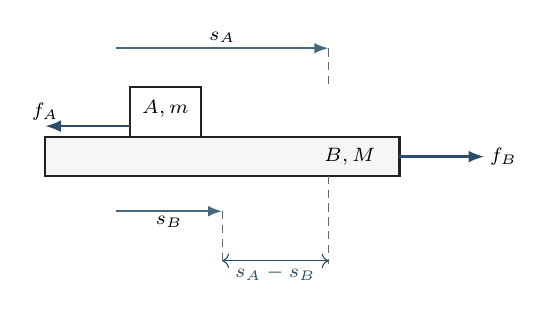
\begin{tikzpicture}[scale=.9]
 \draw[solbody,fill=SoftGray](-2,0)rectangle(3,.55);\node[sollabel]at(2.3,.27){$B,M$};
 \draw[solbody](-.8,.55)rectangle(.2,1.25);\node[sollabel]at(-.3,.95){$A,m$};
 \draw[solforce](-.8,.7)--(-2,.7)node[above,sollabel]{$f_A$};
 \draw[solforce](3,.27)--(4.2,.27)node[right,sollabel]{$f_B$};
 \draw[solflow](-1,1.8)--(2,1.8)node[midway,above,sollabel]{$s_A$};
 \draw[solflow](-1,-.5)--(.5,-.5)node[midway,below,sollabel]{$s_B$};
 \draw[solgeom](.5,-.5)--(.5,-1.25);\draw[solgeom](2,1.8)--(2,1.3);\draw[solgeom](2,0)--(2,-1.25);
 \draw[<->,DeepBlue](.5,-1.2)--(2,-1.2)node[midway,below,sollabel]{$s_A-s_B$};
\end{tikzpicture}\diagcaption{解图}{$A$ 与板接触，摩擦力等大反向；位移箭头比较同一时间内的地面位移。}\label{ch08:fig:soldiagFourFive}\end{workfig}}

\newcommand{\soldiagFourSix}{%
\begin{workfig}\begin{tikzpicture}[scale=.9]
 \foreach \y/\len in {1.8/2.5,0/4.3}{
 \draw[solbody](0,\y)--(5,\y);\draw[solbody,fill=SoftGray](.3,\y)rectangle(1,{\y+.6});
 \draw[solforce](1,{\y+.3})--(2,{\y+.3})node[right,sollabel]{$F$};
 \draw[solflow](.3,{\y-.4})--(\len,{\y-.4});}
 \node[sollabel,anchor=east]at(-.4,2.1){火车系：$0\to u$};
 \node[sollabel,anchor=east]at(-.4,.3){地面系：$v_0\to v_0+u$};
 \node[sollabel,below]at(1.4,1.4){$L$};\node[sollabel,below]at(2.3,-.4){$L+v_0t$};
\end{tikzpicture}\diagcaption{解图}{同一物体、同一时间区间，在两个惯性系中配对比较位移和动能。}\label{ch08:fig:soldiagFourSix}\end{workfig}}

\newcommand{\soldiagFourSeven}{%
\begin{workfig}\begin{tikzpicture}[scale=.9]
 \draw[solbody](-2.5,0)--(3,0);\draw[solbody,fill=SoftGray](-.5,0)rectangle(.5,.8);
 \draw[solforce](.5,.4)--(2,.4)node[right,sollabel]{$F$};
 \draw[solforce](-.5,.4)--(-2,.4)node[left,sollabel]{$ma$};
 \draw[solflow](-1,1.5)--(1,1.5)node[midway,above,sollabel]{火车加速度 $a$};
 \draw[solflow](0,-.5)--(2,-.5)node[midway,below,sollabel]{$L$（$F>ma$）};
\end{tikzpicture}\diagcaption{解图}{惯性力大小 $ma$、方向向左；图示向前位移只对应 $F>ma$ 的分支。}\label{ch08:fig:soldiagFourSeven}\end{workfig}}

\newcommand{\movingPulleyDiagram}{%
\begin{workfig}\begin{tikzpicture}[scale=.9]
 \draw[solbody](.4,2.3)--(1.3,2.3);\draw[solbody](0,0)circle(.8);
 % Rope: left free end, lower semicircle, right fixed end; draw after pulley.
 \draw[DeepBlue,line width=1pt](-.8,1.4)--(-.8,0)arc(180:360:.8)--(.8,2.3);
 \fill(.8,2.3)circle(2pt);\node[sollabel,above]at(.8,2.3){固定端};
 \draw[solbody](0,0)--(0,-1.2);\fill(0,0)circle(2pt);\node[sollabel,above]at(0,.05){轮轴};
 \draw[solbody,fill=SoftGray](-.35,-1.85)rectangle(.35,-1.2);\node[sollabel]at(0,-1.5){$m$};
 \draw[solforce](-.8,1.4)--(-.8,2.35)node[left,sollabel]{$F$};
 \draw[solforce](0,-1.85)--(0,-2.55)node[right,sollabel]{$mg$};
 \draw[solflow](-1.65,.9)--(-1.65,1.9)node[midway,left,sollabel]{$\Delta y_e=L$};
 \draw[solflow](1.55,-.25)--(1.55,.25)node[midway,right,sollabel]{$\Delta y_p=L/2$};
 \node[sollabel,align=left,anchor=west]at(2.3,1.5){蓝线：绕轮缘的绳\\中线：连接轮轴与重物的挂杆};
\end{tikzpicture}\diagcaption{原理图}{位移箭头表示同一过程的上升量，不是某段绳的长度。}\label{ch08:fig:movingPulleyDiagram}\end{workfig}}

\newcommand{\soldiagFourEight}{%
\begin{workfig}\begin{tikzpicture}[scale=.9]
 \draw[solflow](0,0)--(7,0)node[right,sollabel]{$r$};\fill(0,0)circle(3pt)node[below,sollabel]{固定点};
 \fill(1.5,0)circle(2pt)node[below,sollabel]{$r_A$};\fill(5.5,0)circle(2pt)node[below,sollabel]{$r_B$};
 \fill(3.5,0)circle(2pt)node[below,sollabel]{$r$};
 \draw[solforce](3.5,.8)--(2.2,.8)node[midway,above,sollabel]{$\vec F$（向内）};
 \draw[solflow](3.5,-.7)--(4.2,-.7)node[midway,below,sollabel]{$\dd r>0$};
\end{tikzpicture}\diagcaption{解图}{图示向外的一小段位移；引力功微元为 $-(k/r)\dd r$。}\label{ch08:fig:soldiagFourEight}\end{workfig}}

\newcommand{\soldiagFourNine}{%
\begin{workfig}\begin{tikzpicture}[scale=.9]
 \draw[fill=Blue!12,draw=none](1.4,0)--plot[domain=1.4:3.7,samples=60](\x,{1.6/(\x*\x)})--(3.7,0)--cycle;
 \draw[solflow](0,0)--(5,0)node[right,sollabel]{$r$};\draw[solflow](0,0)--(0,3.6)node[above,sollabel]{$F=k/r^2$};
 \draw[solpath,domain=.7:4.7,samples=80]plot(\x,{1.6/(\x*\x)});
 \foreach \r/\name in {1.4/A,3.7/B}{\draw[solgeom](\r,0)--(\r,{1.6/(\r*\r)});\node[sollabel,below]at(\r,0){$r_\name$};}
 \node[sollabel,align=left,anchor=west]at(2,2.2){阴影面积 $=k(1/r_A-1/r_B)$\\[5pt]图示 $r_B>r_A$，故 $W<0$};
\end{tikzpicture}\diagcaption{解图}{阴影是力的大小对距离的积分；功的正负还须结合运动方向。}\label{ch08:fig:soldiagFourNine}\end{workfig}}


\begin{document}
\pagenumbering{arabic}
\setcounter{page}{1}
\setcounter{chapter}{4}
\setcounter{section}{0}

\section{功与功率，动能定理}
\setcounter{equation}{0}

力是改变物体速度的原因。在外力作用下，物体的速度会发生变化。牛顿第二定律集中描述
力与加速度的瞬时关系；在此基础上得到的动量定理，则说明力对时间的积累——冲量——
怎样改变物体的动量。除了动量，还可以用另一个物理量描述运动物体的性质，这就是动能。
本节要建立的核心联系是：力在空间位移上的积累形成“功”，总功等于物体动能的变化。

以下在惯性系中讨论质量不变的质点，$\vec F_{\text{合}}$ 表示它受到的合力。
如图~\ref{ch08:fig:workDerivationDiagram}，质点在 $t$ 时刻位于 $A$，速度为 $\vec v_A$；
经过 $\Delta t$ 到达 $B$，速度为 $\vec v_B$。先定义速度增量
\[
\Delta\vec v=\vec v_B-\vec v_A.
\]
速度有方向，因此应先作矢量相加，再求模的平方，不能直接把速率相加。
\workDerivationDiagram
\begin{equation}
 v_B^2-v_A^2=2\vec v_A\cdot\Delta\vec v+|\Delta\vec v|^2.
 \label{ch08:eq:velocity-square}
\end{equation}
式~\eqref{ch08:eq:velocity-square} 是精确恒等式。若加速度随时间连续，短时间内
$\Delta\vec v=\vec a_A\Delta t+o(\Delta t)$，其中 $o(\Delta t)/\Delta t\to0$。
设 $\vec a_A$ 与 $\vec v_A$ 夹角为 $\theta$，则保留一阶项时
\begin{equation}
 v_B^2-v_A^2=2a_Av_A\cos\theta\,\Delta t+o(\Delta t).
\end{equation}
这里不能把 $|\Delta\vec v|^2$ 当作恒等于零；它在除以 $\Delta t$ 后取极限时才消失。
同样，$\Delta\vec r=\vec v_A\Delta t+o(\Delta t)$，$v_A\Delta t$ 只是小段位移大小的一阶近似。
两边除以 $\Delta t$ 并令 $\Delta t\to0$，再用牛顿第二定律，得到
\begin{equation}
 \frac{\dd}{\dd t}\left(\frac12mv^2\right)
 =m\vec v\cdot\frac{\dd\vec v}{\dd t}
 =\vec F_{\text{合}}\cdot\vec v.
 \label{ch08:eq:kinetic-rate}
\end{equation}
定义动能 $E_k=\tfrac12mv^2$。利用 $\dd\vec r=\vec v\,\dd t$，上式可写成
\begin{equation}
 \dd E_k=\vec F_{\text{合}}\cdot\dd\vec r.
 \label{ch08:eq:differential-work-energy}
\end{equation}
任意力 $\vec F$ 与实际位移微元的夹角为 $\theta$ 时，其功定义为
\begin{equation}
 \dd W=\vec F\cdot\dd\vec r=F\cos\theta\,\dd s,
 \qquad \dd s=|\dd\vec r|.
 \label{ch08:eq:work-element}
\end{equation}
功和动能都是标量，没有空间方向；动能非负，功则可以为正、负或零。
力沿运动方向的分量作正功，反向分量作负功，垂直于瞬时位移的分量不作功。
在有限过程中，把实际路径分段、求和并取分段长度趋于零的极限：
\begin{equation}
 W_{A\to B}=\lim_{\max\Delta s_i\to0}\sum_i\vec F_i\cdot\Delta\vec r_i
 =\int_A^B\vec F\cdot\dd\vec r.
 \label{ch08:eq:work-integral}
\end{equation}
将式~\eqref{ch08:eq:differential-work-energy} 沿同一过程积分，中间状态的动能增减相互衔接，得到
\begin{equation}
 W_{\text{合}}(A\to B)=E_{k,B}-E_{k,A}
 =\frac12mv_B^2-\frac12mv_A^2.
 \label{ch08:eq:work-energy}
\end{equation}
合力功等于各分力功的代数和。总功为正，
物体动能增加；总功为负，物体动能减小。直观地说，沿运动方向推物体通常使其速率增大，
逆着运动方向施力通常使其速率减小；但严格判断仍应以力与位移的夹角以及全过程功的
代数和为准。

\subsection{功和动能的确定}

应用动能定理可以使许多问题大为简化，但必须先明确研究对象、过程的初末状态，以及各力
所做功的正负。对恒力而言，只有力在位移方向上的分量做功；垂直于位移的力不做功。

\subsubsection*{恒力功、功率与动能定理的使用范围}

恒力的大小和方向都不变，可从式~\eqref{ch08:eq:work-integral} 的积分号内提出：
\[
 W=\vec F\cdot\int_A^B\dd\vec r
  =\vec F\cdot(\vec r_B-\vec r_A)=F|\vec r_B-\vec r_A|\cos\theta.
\]
这里用的是始末位置之间的位移，不是弯曲路径的长度。变力一般不能这样提出积分号，必须沿实际路径计算。
点积还说明只有切向分量作功；法向力即使很大也可能不作功，但它仍可改变速度方向。

功率表示作功的快慢。时间间隔 $\Delta t$ 内的平均功率为 $\overline P=W/\Delta t$；令时间间隔趋于零，得到瞬时功率
\begin{equation}
 P=\frac{\dd W}{\dd t}
 =\vec F\cdot\frac{\dd\vec r}{\dd t}
 =\vec F\cdot\vec v=F_t v.
 \label{ch08:eq:power}
\end{equation}
$F_t$ 是力沿速度方向的有符号分量。功的单位是焦耳，$1\,\mathrm J=1\,\mathrm{N\,m}$；功率单位是瓦特，
$1\,\mathrm W=1\,\mathrm{J/s}$。只有牵引力平行于速度且 $v>0$ 时，才能由此写成 $F=P/v$。
因此匀功率与恒牵引力不是同一条件：匀功率时速度升高，牵引力减小。不能把这个理想关系直接外推到静止启动瞬间；实际机器的牵引力有上限。

也可以在直角坐标中逐项验证式~\eqref{ch08:eq:kinetic-rate}。把牛顿第二定律的三个分量分别乘以相应速度分量，再相加：
\begin{align*}
 F_xv_x+F_yv_y+F_zv_z
 &=m\left(v_x\frac{\dd v_x}{\dd t}+v_y\frac{\dd v_y}{\dd t}+v_z\frac{\dd v_z}{\dd t}\right)\\
 &=\frac{\dd}{\dd t}\left[\frac m2(v_x^2+v_y^2+v_z^2)\right]
 =\frac{\dd E_k}{\dd t}.
\end{align*}
再乘 $\dd t$ 并积分，左边利用 $v_x\dd t=\dd x$ 等关系化为合力功，右边成为末动能减初动能。
所以动能定理是牛顿第二定律沿实际路径的积分形式，适于联系速率和位置；若还要求时间或速度方向，通常要配合运动学或分量方程。

对质点系，外力功与内力功共同决定总动能变化。两个物体间作用力等大反向，但其作用点位移一般不同，
所以内力总功未必为零；弹簧伸缩、碰撞形变和摩擦发热都体现了这一点。只有把内力功转化为相应势能或内能，
才能写成更完整的能量关系。参考系改变时速度、动能和功都会改变，但在同一惯性系中二者始终满足动能定理。

虚功方法研究满足约束的假想无穷小位移。理想约束力对允许的虚位移的总功为零，平衡时主动外力的总虚功也为零。
它把合力、合力矩平衡改写到约束允许的坐标中，常能避开未知支持力和绳张力；后文将用动滑轮说明。


\begin{origexamplebox}{例 4.1}
以下各图中 $A,B$ 两点的高度差均为 $h$。物体分别沿图示各条路径由 $A$ 到 $B$，
求每一过程中重力所做的功。
\probdiagFourOne
\end{origexamplebox}

\begin{xesolution}
图~\ref{ch08:fig:probdiagFourOne} 的各条路径具有同一高度差；在图~\ref{ch08:fig:soldiagFourOne} 中把端点记为 $y_A,y_B$。
取竖直向上为 $y$ 轴正方向。重力为 $\vec G=-mg\,\vec e_y$，任意一小段位移中重力做功
\[
 \dd W_G=\vec G\cdot\dd\vec r=-mg\,\dd y.
\]
从 $A$ 到 $B$ 累积：
\[
 W_G=-mg\int_{y_A}^{y_B}\dd y
 =mg(y_A-y_B).
\]
\soldiagFourOne
由于所有图中 $y_A-y_B=h$，无论路径是直线、折线、曲线，途中是否先升高或绕行，
均有
\[
 \boxed{W_G=mgh}.
\]
重力功只由初、末位置的高度差决定，与实际路径的形状和长度无关。
\end{xesolution}

\Needspace{0.34\textheight}
\begin{origexamplebox}{例 4.2}
质量为 $m$ 的物体在与水平方向夹角为 $\theta$ 的恒力 $F$ 作用下，沿摩擦系数为
$\mu$ 的水平面向右运动距离 $L$。求在此过程中恒力 $F$、摩擦力 $f$、重力 $mg$
以及支持力 $N$ 所做的功。若初速度为 $v_0$、方向向右，求物体最后的速度。
\probdiagFourTwo
\end{origexamplebox}

\begin{xesolution}
图~\ref{ch08:fig:probdiagFourTwo} 给出 $F$ 与水平线的夹角，图~\ref{ch08:fig:soldiagFourTwo} 分别标出四个力。
物体在竖直方向没有位移。若全过程保持与水平面接触，则
\[
 N+F\sin\theta-mg=0,
 \qquad
 N=mg-F\sin\theta.
\]
滑动摩擦力大小为
\[
 f=\mu N=\mu(mg-F\sin\theta),
\]
方向与位移相反。各力所做的功分别为
\[
 \boxed{W_F=FL\cos\theta},
 \qquad
 \boxed{W_f=-\mu(mg-F\sin\theta)L},
\]
\[
 \boxed{W_G=0},
 \qquad
 \boxed{W_N=0}.
\]
\soldiagFourTwo
对物体应用动能定理：
\[
 FL\cos\theta-\mu(mg-F\sin\theta)L
 =\frac12mv^2-\frac12mv_0^2.
\]
所以
\[
 \boxed{
 v=\sqrt{v_0^2+\frac{2L}{m}
 \left[F\cos\theta-\mu(mg-F\sin\theta)\right]}}.
\]
这一表达式要求 $N\ge0$，且物体确实向右滑完整段距离 $L$。若根号内在到达 $L$ 前
已降为零，物体会先停下，摩擦力方向和后续运动必须重新判断。
\end{xesolution}

\Needspace{0.35\textheight}
\begin{origexamplebox}{例 4.3}
如图，质量为 $m$ 的小球系在劲度系数为 $k$、原长为 $l_0$ 的轻弹簧一端，弹簧另一端
固定在 $O$ 点。开始时小球位于水平位置 $A$，弹簧处于原长。小球由 $A$ 自由释放，
下落到 $O$ 点正下方的 $B$ 点时，弹簧伸长量为 $l_0/n$，其中 $n>0$。已知小球能够到达该状态，求其速率。
\probdiagFourThree
\end{origexamplebox}

\begin{xesolution}
图~\ref{ch08:fig:probdiagFourThree} 标出两个状态，虚线只连接始末位置，不用于指定运动轨迹。
在 $A$ 点弹簧长度为原长 $l_0$，在 $B$ 点弹簧长度为
\[
 OB=l_0+\frac{l_0}{n}=l_0\left(1+\frac1n\right).
\]
因此小球下降的高度就是 $OB$。重力做功
\[
 W_G=mg\,l_0\left(1+\frac1n\right).
\]
令弹簧伸长量为 $x=l-l_0$，径向向外为正。弹力为 $-kx\vec e_r$，
而实际位移在径向上的投影为 $\dd l=\dd x$，所以即使轨迹弯曲，也有
\[
 \dd W_{\rm s}=(-kx\vec e_r)\cdot\dd\vec r=-kx\,\dd x.
\]
从 $x=0$ 积分到 $x=l_0/n$，得到
\[
 W_{\rm s}=-\int_0^{l_0/n}kx\,\dd x=-\frac12k\left(\frac{l_0}{n}\right)^2.
\]
图~\ref{ch08:fig:soldiagFourThree} 将高度差和形变量分开标出，分别用于计算重力功和弹力功。
\soldiagFourThree
小球由静止释放，由动能定理
\[
 mg\,l_0\left(1+\frac1n\right)
 -\frac12k\frac{l_0^2}{n^2}
 =\frac12mv^2.
\]
故
\[
 \boxed{
 v=\sqrt{2gl_0\left(1+\frac1n\right)
 -\frac{k l_0^2}{mn^2}}}.
\]
弹力虽然在曲线路径上方向不断改变，但其总功只由弹簧初、末形变量决定。
根号内各项量纲均为速度平方。它必须非负；题给的 $n$ 是实际到达状态的参数，不能把任意 $n$ 都当作必可实现的运动状态。
\end{xesolution}

\subsection{多个物体的情况}

动能定理不但适用于单个质点，也适用于由多个质点构成的力学系统。系统的总动能等于
各质点动能的代数和。与动量定理不同，系统内力的总功一般不为零；求系统总动能的变化
时，外力功和内力功都不能遗漏。例如枪和子弹的总动量在发射过程中可以守恒，但火药内力
做正功，使系统总动能明显增加。

\Needspace{0.32\textheight}
\begin{origexamplebox}{例 4.4}
如图，把弹簧的一端固定在墙上，另一端系物体 $A$。将弹簧压缩 $x_1$ 后，在 $A$ 的
右边紧靠放置物体 $B$，然后撤去外力。物体 $A,B$ 均在光滑水平面上，质量分别为
$m_A,m_B$，弹簧劲度系数为 $k$。求物体 $A$ 移动的最大距离。
\probdiagFourFour
\end{origexamplebox}

\begin{xesolution}
按图~\ref{ch08:fig:probdiagFourFour}，以弹簧连接点在原长时的位置为 $x=0$，伸长为正。
弹簧由压缩状态恢复时，$A$ 推着 $B$ 一起向右运动。在弹簧仍被压缩的阶段，两物体速度
相同，可看作总质量为 $m_A+m_B$ 的整体。此时 $x<0$，共同加速度及 $A$ 对 $B$ 的接触力为
\[
 a=\frac{-kx}{m_A+m_B},\qquad N=m_Ba=\frac{-m_Bkx}{m_A+m_B}>0.
\]
因此在恢复原长之前不会分离；到 $x=0$ 时 $N$ 才降为零。由动能定理
\[
 \frac12kx_1^2
 =\frac12(m_A+m_B)V^2,
\]
故
\[
 V=x_1\sqrt{\frac{k}{m_A+m_B}}.
\]
越过原长位置后，弹簧开始伸长并向左拉 $A$，而 $A$ 不能“拉住”右侧的 $B$，所以两物体
在弹簧原长处恰好分离。此后 $B$ 以速度 $V$ 匀速前进，$A$ 单独继续向右并拉伸弹簧。
\soldiagFourFour
图~\ref{ch08:fig:soldiagFourFour} 的三行分别表示初态、分离和 $A$ 到达最右端；三行使用相同的 $x=0$。
设 $A$ 在原长位置右侧继续移动的最大距离为 $x_2$，则
\[
 \frac12m_AV^2=\frac12kx_2^2,
\]
从而
\[
 x_2=x_1\sqrt{\frac{m_A}{m_A+m_B}}.
\]
物体 $A$ 从初始压缩位置到最右端的总路程为 $x_1+x_2$，所以
\[
 \boxed{
 s_{A,\max}=x_1\left(1+\sqrt{\frac{m_A}{m_A+m_B}}\right)}.
\]
若只问相对弹簧原长位置的最大伸长，则答案是 $x_2$；本题问的是 $A$ 从初始位置起移动的
最大距离，因此还要加上先前走过的 $x_1$。
\end{xesolution}

\Needspace{0.28\textheight}
\begin{origexamplebox}{例 4.5}
光滑水平面上有一块足够长、质量为 $M$、初始静止的板 $B$。某时刻质量为 $m$、
速度为 $v_0$ 的物体 $A$ 冲上板的上表面，两者间的动摩擦因数为 $\mu$。求从开始相对
滑动到相对速度变为零的过程中，摩擦力对两个物体所做的功各为多少；并求整个系统的
动能变化量。
\end{origexamplebox}

\begin{xesolution}
水平方向没有外力，达到共同速度 $V$ 时由动量守恒
\[
 mv_0=(m+M)V,
 \qquad
 V=\frac{m}{m+M}v_0.
\]
滑动期间，$A$ 的加速度为 $-\mu g$，板 $B$ 的加速度为 $\mu mg/M$。相对速度由
$v_0$ 减到零。相对加速度为两加速度之差，故
\[
 a_{A/B}=-\mu g-\frac{\mu mg}{M},\qquad
 0=v_0-\mu g\left(1+\frac mM\right)t.
\]
所需时间为
\[
 t=\frac{Mv_0}{\mu g(m+M)}.
\]
两物体相对地面的位移分别为
\[
 s_A=\frac{v_0+V}{2}\,t,
 \qquad
 s_B=\frac{V}{2}\,t.
\]
\soldiagFourFive
图~\ref{ch08:fig:soldiagFourFive} 中 $s_A>s_B$，两位移都相对地面计算。
摩擦力对 $A$ 方向向左，对 $B$ 方向向右，因此
\[
 \boxed{
 W_{f,A}=-\mu mgs_A
 =-\frac{mM(M+2m)}{2(m+M)^2}v_0^2},
\]
\[
 \boxed{
 W_{f,B}=+\mu mgs_B
 =\frac{m^2M}{2(m+M)^2}v_0^2}.
\]
系统动能变化为两摩擦功之和：
\[
 \boxed{
 \Delta E_k=W_{f,A}+W_{f,B}
 =-\frac{mM}{2(m+M)}v_0^2}.
\]
两个摩擦力大小相等、方向相反，但作用点相对地面的位移不同，所以它们的功不互相抵消。
损失的机械能等于摩擦力与相对滑动距离的乘积。也可分别核验
$W_{f,A}=\tfrac12m(V^2-v_0^2)$、$W_{f,B}=\tfrac12MV^2$，代入共同速度即得到同样结果。
这里取 $\mu>0$；减小 $\mu$ 会延长滑动时间，最终损失却不变，而 $\mu=0$ 时根本不会达到共同速度，不能套用这一终态。
\end{xesolution}

\subsection{不同参考系中的动能定理}

功依赖于力的作用点在所选参考系中的位移，动能依赖于物体在所选参考系中的速度，因此
二者都与参考系有关。只有在惯性参考系中，动能定理才能直接写成通常形式；同一过程可以
在不同惯性系中使用动能定理，但必须在同一个参考系内同时计算功和动能。

\begin{origexamplebox}{例 4.6}
一列火车以速度 $v_0$ 做匀速直线运动。火车上的人在光滑水平面上用恒力 $F$ 向前拉动质量为 $m$ 的物体，
使它相对火车向前移动距离 $L$。物体起初相对火车静止。先在火车参考系中求物体最后的
速度，再在相对地面静止的参考系中描述同一过程，并列出动能定理方程。
\end{origexamplebox}

\begin{xesolution}
火车做匀速直线运动，火车系与地面系都是惯性系。设物体相对火车的末速度为 $u$。在火车
系中，力的作用点位移为 $L$，动能定理给出
\[
 FL=\frac12mu^2,
 \qquad
 \boxed{u=\sqrt{\frac{2FL}{m}}}.
\]
设拉动持续时间为 $t$。由于 $u=Ft/m$，所以 $m u=Ft$。在地面系中，物体的初、末速度
分别为 $v_0$ 和 $v_0+u$；同一时间内，力的作用点相对地面的位移为 $L+v_0t$。
\soldiagFourSix
图~\ref{ch08:fig:soldiagFourSix} 的两行对应同一过程：地面位移等于车内位移加上火车的位移。
地面系中的动能定理为
\[
 \boxed{
 F(L+v_0t)
 =\frac12m(v_0+u)^2-\frac12mv_0^2}.
\]
展开右端并利用 $FL=\tfrac12mu^2$、$Ft=mu$，两边完全相等。不同惯性系中功和动能
变化的数值可以不同，但各自在本参考系内仍满足动能定理。
\end{xesolution}

\Needspace{0.30\textheight}
\begin{origexamplebox}{例 4.7}
同上，但火车以加速度 $a$ 做匀加速运动。在火车参考系和地面参考系中分别直接使用
动能定理，能否得到正确结果？若要使动能定理在火车参考系中也成立，应怎样处理？
\end{origexamplebox}

\begin{xesolution}
地面系近似为惯性系，因而可以直接使用动能定理。设过程开始时火车和物体的地面速度均为
$v_0$，持续时间为 $t$。物体只受水平拉力 $F$，故地面加速度为 $F/m$：
\[
 v_{\rm f}=v_0+\frac{F}{m}t,
 \qquad
 x_{\rm obj}=v_0t+\frac12\frac{F}{m}t^2.
\]
地面系中有
\[
 \boxed{
 Fx_{\rm obj}
 =\frac12m\left(v_0+\frac{F}{m}t\right)^2-\frac12mv_0^2}.
\]
火车系以加速度 $a$ 运动，不是惯性系。若仍只把 $F$ 的功写成 $FL$，将不能得到正确的
相对运动。要在火车系中使用动能定理，必须给物体加入方向与火车加速度相反的惯性力
\[
 \vec F_{\rm in}=-m\vec a.
\]
\soldiagFourSeven
图~\ref{ch08:fig:soldiagFourSeven} 中真实拉力向右、惯性力向左。
若拉力与火车加速度同向，且 $F>ma$，物体相对火车由静止向前移动距离 $L$，则
\[
 (F-ma)L=\frac12mu_{\rm rel}^2,
\]
所以
\[
 \boxed{u_{\rm rel}
 =\sqrt{2\left(\frac{F}{m}-a\right)L}}.
\]
若 $F=ma$，相对加速度为零，物体始终相对火车静止，不会完成 $L>0$ 的车内位移。
若 $F<ma$，物体相对火车向后运动；用有符号位移 $\xi<0$ 写
$(F-ma)\xi=\tfrac12mu_{\rm rel}^2$，两边仍为非负，不能把“向前移动 $L$”的根式硬套到此分支。
惯性力不是新的相互作用力，而是为了在非惯性系中继续使用牛顿定律和动能定理而引入的
等效力。
\end{xesolution}

\subsection{功与力的关系：虚功原理初步}

杠杆、轮轴、齿轮、定滑轮和动滑轮
等简单机械可以组合成复杂装置，把动力转化为所需要的形式。机械的一端连接动力源，动力
可以来自人力、蒸汽机或电动机；另一端是输出端，用来提升重物或产生其他运动。

机械不能创造能量，但可以储存能量。无摩擦、无其他损耗时，输入功与输出功的正确关系是
\[
 W_{\rm in}=W_{\rm out}+\Delta E_{\rm machine}.
\]
只有机械本身的动能、势能等不变时，才有输入功等于输出功；无摩擦本身并不能保证这一点。
在这个条件下，机械用较小的力克服较大的阻力，代价是动力作用点移动更长的距离，“省力”不意味着“省功”。

图~\ref{ch08:fig:movingPulleyDiagram} 为轻绳、轻滑轮构成的理想动滑轮，绳不可伸长，下方重物质量为 $m$。
取竖直向上为正，固定端高度为 $y_f$，自由端高度为 $y_e$，轮心高度为 $y_p$。
绳长为 $(y_f-y_p)+(y_e-y_p)+\pi R=\text{常量}$，所以
$\Delta y_e=2\Delta y_p$。自由端向上移动 $L$ 时，重物向上移动 $L/2$。
重物匀速上升，动能不变，因此拉力的功等于重力势能的增加：
\movingPulleyDiagram
\begin{equation}
 F L=mg\frac{L}{2}.
\end{equation}
消去共同的位移尺度 $L$，得到
\begin{equation}
 F=\frac12mg.
\end{equation}
如果装置处于平衡而并未实际运动，也可以假想一次符合绳长约束的微小位移，记作 $\delta y$。
它不是已经发生的位移，也不要求给它分配一段时间。理想约束下，平衡要求主动外力的总虚功为零：
\[
 F\delta y_e-mg\delta y_p=0,\qquad \delta y_e=2\delta y_p.
\]
由此同样得到 $F=mg/2$。这就是虚功原理在本例中的用法。
它把允许的位移关系与平衡条件结合起来，可避免逐个求出约束复杂系统中的支持力和内部绳张力。

\subsection{变力作功}

作用力不是恒力时，仍可使用动能定理，关键是正确计算变力的功。建立直角坐标系，把力写成
$(F_x,F_y,F_z)$，位移微元写成 $(\dd x,\dd y,\dd z)$，则功的微元为
\begin{equation}
 \dd W=F_x\dd x+F_y\dd y+F_z\dd z=\vec F\cdot\dd\vec r.
\end{equation}
在有限过程中，应把各微小功累积起来，即
\[
 W=\int_A^B\vec F\cdot\dd\vec r.
\]

\Needspace{14\baselineskip}
\begin{origexamplebox}{例 4.8}
两个物体间的相互吸引力大小与它们之间的距离成反比。固定其中一个物体，求另一个物体
由相距 $r_A$ 运动到相距 $r_B$ 的过程中，该吸引力所做的功。
\end{origexamplebox}

\begin{xesolution}
设吸引力大小为
\[
 F=\frac{k}{r},
 \qquad k>0.
\]
取径向向外为正方向，吸引力的径向分量为 $F_r=-k/r$。因此
\[
 W_{A\to B}
 =\int_{r_A}^{r_B}F_r\,\dd r
 =-\int_{r_A}^{r_B}\frac{k}{r}\,\dd r.
\]
\soldiagFourEight
图~\ref{ch08:fig:soldiagFourEight} 区分有限的始末距离与当前位置上的径向位移微元。积分得到
\[
 \boxed{W_{A\to B}=k\ln\frac{r_A}{r_B}}.
\]
若题目所说“大小”专指绝对值，则为
\[
 \boxed{|W|=k\left|\ln\frac{r_A}{r_B}\right|}.
\]
当物体向内运动，即 $r_B<r_A$ 时，引力与位移同向，功为正；向外运动时功为负。
\end{xesolution}

\begin{origexamplebox}{例 4.9}
两个物体间的相互吸引力大小与它们之间距离的平方成反比。固定其中一个物体，求另一个
物体由相距 $r_A$ 运动到相距 $r_B$ 的过程中，该吸引力所做的功。
\end{origexamplebox}

\begin{xesolution}
设吸引力大小为
\[
 F=\frac{k}{r^2},
 \qquad k>0.
\]
仍取径向向外为正，故 $F_r=-k/r^2$：
\[
 W_{A\to B}
 =-\int_{r_A}^{r_B}\frac{k}{r^2}\,\dd r
 =\left.\frac{k}{r}\right|_{r_A}^{r_B}.
\]
\soldiagFourNine
图~\ref{ch08:fig:soldiagFourNine} 画出 $r_B>r_A$ 时力的大小曲线：阴影面积为正，而向外运动的引力功为负。
所以功及其绝对值分别为
\[
\boxed{
 W_{A\to B}=k\left(\frac1{r_B}-\frac1{r_A}\right)},
\qquad
\boxed{
 |W|=k\left|\frac1{r_B}-\frac1{r_A}\right|}.
\]
符号判断与例 4.8 相同：向内运动时引力做正功，向外运动时引力做负功。
\end{xesolution}

\end{document}
